\documentclass[12pt]{article}
\usepackage{bussproofs, array, amstext, amssymb} 
\usepackage{mathtools, extarrows}
\usepackage{latexsym}
\usepackage{syntax}
\usepackage{tabularx}
\usepackage{flowchart}
\usepackage{array,multirow}
\usepackage[section]{placeins}
\usepackage[bottom]{footmisc}
% \usepackage[charter]{mathdesign}
\usepackage{tablefootnote}
\usepackage[nodayofweek,level]{datetime}
\usepackage[affil-it]{authblk}
\usepackage{hyperref}
\usepackage{algorithm,algpseudocode}
\usepackage{textcomp}
\usepackage{pgfplots}
\usepackage[utf8]{inputenc}
\usepackage[T1]{fontenc}
\usepackage{catchfilebetweentags}
\usepackage{agda}
\usepackage[verbose]{newunicodechar}

\newunicodechar{ᵇ}{\ensuremath{\mathnormal{\sp{b}}}}
\newunicodechar{⊎}{\ensuremath{\mathnormal{\uplus}}}
\newunicodechar{₁}{\ensuremath{\mathnormal{\sb{1}}}}
\newunicodechar{₂}{\ensuremath{\mathnormal{\sb{2}}}}
\newunicodechar{≤}{\ensuremath{\mathnormal{\le}}}
\newunicodechar{≈}{\ensuremath{\mathnormal{\approx}}}
\newunicodechar{∀}{\ensuremath{\mathnormal{\forall}}}
\newunicodechar{∃}{\ensuremath{\mathnormal{{\exists}}}}
\newunicodechar{≡}{\ensuremath{\mathnormal{\equiv}}}
\newunicodechar{Γ}{\ensuremath{\mathnormal{\Gamma}}}
\newunicodechar{λ}{\ensuremath{\mathnormal{\lambda}}}
\newunicodechar{ϕ}{\ensuremath{\mathnormal{\phi}}}
\newunicodechar{ψ}{\ensuremath{\mathnormal{\psi}}}
\newunicodechar{∷}{\ensuremath{\mathnormal{::}}}
\newunicodechar{⊤}{\ensuremath{\mathnormal{\top}}}
\newunicodechar{⊥}{\ensuremath{\mathnormal{\bot}}}
\newunicodechar{∨}{\ensuremath{\mathnormal{\lor}}}
\newunicodechar{∧}{\ensuremath{\mathnormal{\land}}}
\newunicodechar{→}{\ensuremath{\mathnormal{\to}}}
\newunicodechar{↔}{\ensuremath{\mathnormal{\leftrightarrow}}}
\newunicodechar{⇒}{\ensuremath{\mathnormal{\Leftarrow}}}
\newunicodechar{⇔}{\ensuremath{\mathnormal{\Leftrightarrow}}}
\newunicodechar{∈}{\ensuremath{\mathnormal{\in}}}
\newunicodechar{≠}{\ensuremath{\mathnormal{\neq}}}
\newunicodechar{≠}{\ensuremath{\mathnormal{\neq}}}
\newunicodechar{ʳ}{\ensuremath{\mathnormal{\sp{r}}}}
\newunicodechar{⊨}{\ensuremath{\mathnormal{\vDash}}}
\newunicodechar{↦}{\ensuremath{\mathnormal{\mapsto}}}
\newunicodechar{∘}{\ensuremath{\mathnormal{\circ}}}

 

\pgfplotsset{compat=1.14}
\definecolor{verif}{HTML}{019529}
\definecolor{fast}{HTML}{0C06F7}

\algrenewcommand{\algorithmiccomment}[1]{\hskip3em$\rhd$ #1}
\algdef{SE}[SUBALG]{Indent}{EndIndent}{}{\algorithmicend\ }%
\algdef{SE}[SWITCH]{Case}{EndCase}[1]{\textbf{case}\ #1\ \textbf{of}}{\algorithmicend\ \algorithmicswitch}%
\algtext*{Indent}
\algtext*{EndIndent}
\algtext*{EndCase}
\algtext*{EndFor}% Remove "end for" text
\algtext*{EndWhile}% Remove "end while" text
\algtext*{EndIf}% Remove "end if" text
\algtext*{EndFunction}% Remove "end if" text

\renewcommand{\labelitemii}{$\star$}
\newcommand{\midtilde}{\raisebox{0.5ex}{\texttildelow}}
\newcommand{\at}[0]{\ @\ }
\newcommand{\An}[0]{\mathrm{An}}
\newcommand{\len}[0]{\mathrm{len}}
\newcommand{\Gnd}[0]{\mathit{gnd}}
\newcommand{\Prf}[0]{\mathit{prf}}
\newcommand{\Bch}[0]{\mathit{bch}}
\newcommand{\Bchs}[0]{\mathit{bchs}}
\newcommand{\Prob}[0]{\mathit{prob}}
\newcommand{\idf}[1]{\#_{#1}} 
\newcommand{\fresh}[1]{\mathit{fresh}_{\#}({#1})} 
\newcommand{\mfi}[0]{\mathrm{mfi}} 
\newcommand{\Dec}[1]{\xRightarrow{#1}} 
\newcommand{\bprf}[0]{\begin{prooftree}}
\newcommand{\eprf}[0]{\end{prooftree}}
\newcommand{\axm}[1]{\AxiomC{$#1$}}
\newcommand{\unr}[1]{\UnaryInfC{$#1$}}
\newcommand{\bnr}[1]{\BinaryInfC{$#1$}}
\newcommand{\tnr}[1]{\TrinaryInfC{$#1$}}
\newcommand{\rlb}[1]{\RightLabel{#1}}
\newcommand{\limp}[0]{\to}
\newcommand{\liff}[0]{\leftrightarrow}
\newcommand{\sq}[1]{\text{`#1'}} 

\newcommand{\size}[0]{\mathrm{size}}
\newcommand{\lfi}[0]{\mathrm{lfi}} 
\newcommand{\adm}[0]{\mathrm{adm}}

 
\newcommand{\concat}{%
  \mathbin{{+}\mspace{-8mu}{+}}%
}

\makeatletter
\def\@maketitle{%
  \newpage
  \null
  \vskip 2em%
  \begin{center}%
  \let \footnote \thanks
    {\Large\bfseries \@title \par}%
    \vskip 1.5em%
    {\normalsize
      \lineskip .5em%
      \begin{tabular}[t]{c}%
        \@author
      \end{tabular}\par}%
    \vskip 1em%
    {\normalsize \@date}%
  \end{center}%
  \par
  \vskip 1.5em}
\makeatother

\title{A Formally Verified TESC Verifier}

\author{Seulkee Baek}

\begin{document}

\maketitle

\begin{abstract}

This paper introduces the Verified TESC Verifier (VTV), a formally verified 
checker for the new Theory-Extensible Sequent Calculus (TESC) proof format for first-order ATPs. VTV accepts a
TPTP problem and a TESC proof as input, and uses the latter to verify the 
unsatisfiability of the former. VTV is written in Agda, and the soundness 
of its proof-checking kernel is verified in respect to a first-order
semantics formalized in Agda. VTV shows robust performance in a comprehensive 
test using all elligible problems from the TPTP problem library, 
successfully verifying all but the 3 largest proofs out of 12296 proofs,
with >97\% of the proofs verified under 1 second. 




\end{abstract}


\section{Introduction}

Modern automated reasoning tools are highly complex software whose correctness 
cannot be easily established. Numerous bugs have been discovered in them
in the past, and more are presumably hidden in sytems used today. One popular 
strategy for coping with the possibility of errors in automated reasoning is the 
\textit{De Brujin} criterion \cite{barendregt2005challenge}, which states that 
automated reasoning software should produce `proof objects' which can be 
independently verified by simple checkers that users can easily understand 
and trust. In addition to reducing the trust base of theorem provers, 
adherence to the De Bruijn criterion comes with the additional benefit that the 
small trusted core is often simple enough to be formally verified themselves. 
Such thoroughgoing verification is far from universal, but there has been notable 
progress toward this goal in various subfields of automated reasonning, 
including interactive theorem provers, SAT solvers, and SMT solvers.

One area in which similar developments have been conspicuously absent is 
first-order automated theorem provers (ATPs), where the lack of a machine-checkable
proof format precluded any simple independent verifiers, much less a
formally verified one. The Theory-Extensible Sequent Calculus (TESC) is a new 
proof format for first-order ATPs designed to address this gap. In particular,
the format's small set of fined-grained inference rules makes it 
straightforward to implement and verify its proof checker.

This paper presents the Verified TESC Verifier (VTV), a proof checker for  
the TESC format written and verified in Agda \cite{}. 
The aim of the paper is twofold:
primary aim = provide confidence in the TESC proof format. The statement and 
proof of VTV's soundness shows exactly what is entailed by a successful
verification of a TESC proof. Hopes of increased developer interest in the new format 
Secondary aim = a guide for understanding the VTV codebase and possibly implementing 
your own TESC verifier, especially in dependently typed languages such as Lean or Coq.

The rest of the paper is organized as follows:
Section \ref{sec:format} describes the syntax and inference rules 
of the TESC proof calculus.
Section \ref{sec:verifier} presents the main TESC verifier, and
Section \ref{sec:correctness} deals with the statement and proof of verifier
correctness. 
Sections \ref{sec:format}, \ref{sec:verifier}, and \ref{sec:correctness} 
are also accompanied by code excerpts and discussions of the Agda 
formalization of their respective contents. 
Section \ref{sec:test-results} shows results of empirical tests that compare 
the performance of VTV against the default TESC verifier written in Rust. 
Section \ref{sec:rel-works} briefly surveys related works. Section 
\ref{sec:conclusion} gives a summary and discusses potential future work.

\section{Related Works} \label{sec:rel-works}

SAT solving is arguably the most developed subfield of automated reasoning
in terms of proof checker certification. A non-exhaustive list of verified 
verifiers for SAT proof formats include... 

Despite the hard limits imposed by Goedel's second incompleteness theorem \cite{},
there has been interesting work toward self-verification of interactive 
theorem prover kernels. All of HOL Light except the axiom of infinity has been 
proven consistent in HOL Light itself \cite{}, which allows us to consider HOL Light
consistent for most practical proofs (i.e., any proof that is not artificially 
contrived to exploit the missing axiom). More recent work on Metamath Zero \cite{}
aims to verify not only a large part of Metamath Zero's logic, but also its 
implementation down to the level of x84-64 instruction set architecture. 

The SMTCoq project \cite{} also includes a checker for SMT proofs that has been 
formally verified in and extracted from Coq.

VTV is designed to serve a role similar to these verified checkers for first-order ATPs
and the TESC format.
There has been several different approaches to verifying the output of ATPs, but (to the
extent of my knowledge) none has featured a proof format with a verified checker. 
For instance, GDV \cite{} works by breaking down an ATP-generated solution into small 
subproblems and re-solving them with multiple ATPs. The redundancy of multiple ATPs 
provides more reliability than any single solver, but there isn't much that can be 
verified about the operation of GDV short of verifying the highly complex ATPs used.  
Foundational Proof Certificates \cite{} is a system that could potentially be used to 
specify proof formats and implement proof checkers for first-order ATPs, but its actual 
implementation has been limited to specification of the paramodulation rule and an 
unverified checker.



















The self-verification of HOL Light showed that 





 Verified LRAT checkers, self-verification of HOL Light and Metamath-0


\section{Conventions}



`Its largest functor index is smaller than its size'' is a mouthful, we 
simply say that a sequent $\Gamma$ is \textit{good} iff $\lfi(\Gamma) < \size(\Gamma)$.

Define 'functor'
Define 'DTV'

\section{Proof Calculus} \label{sec:format} 

As its name suggests, the TESC proof format is based on a first-order 
sequent calculus. Compared to typical first-order sequent calculi, the
TESC calculus includes some oddities which facilitates mechanical proof 
construction and verification. The syntax of TESC terms and formulas are 
as follows:
\begin{align*}
f ::= &\ \sigma\ |\ \idf{k}\\
t ::= &\ x_k\ |\ f(\vec{t})\\
\vec{t} ::= &\ \cdot\ |\ t, \vec{t}\\
\phi ::= &\ \top\ |\ \bot\ |\ f(\vec{t})\ |\ \lnot \phi\ |\ \phi \lor \chi\ |\ \phi \land \chi\ |\ \phi \to \chi\ |\ \phi \leftrightarrow \chi\ |\ \forall \phi\ |\ \exists \phi
\end{align*}
$t$ ranges over terms, $\vec{t}$ over lists of terms, and $\phi$ over formulas.
Quantified formulas are written without variables due to the use of De Bruijn 
indices \cite{}; the number $k$ in variable $x$ is its De Bruijn index. 
$f$ and $r$ are regular function and relation symbols. Symbols of the 
form $\idf{k}$ are \textit{indexed functors}, a special syntactic class
which may be used as either function or relation symbols. The number $k$ of 
a indexed functor $\idf{k}$ is its \textit{functor index}. Indexed 
functors are used to ensure that a newly introduced function or relation 
symbol is fresh: if you know that $k$ is the largest functor index that 
occurs in the current environment, you may safely use $\idf{k+1}$ as a 
fresh symbol without having to search through the enviroment.

Formalization of TESC syntax in Agda is mostly straightforward, but with one 
caveat: the first-instinct definition of terms as 
\ExecuteMetaData[wrongterm.tex]{wrongterm}
works poorly in practice, since any structural recursion on terms immediately 
runs into non-termination issues. We could try to manually prove termination,
but it is much simpler to sidestep this issue with a pseudo-mutual recursion:
\ExecuteMetaData[basic.tex]{termstar}
which lets us define terms and lists of terms as
\ExecuteMetaData[basic.tex]{termterms}

\begin{table}
  \begin{tabular}{|c|c|} \hline
  Rule & Conditions \\ \hline
  \multirow{2}{*}{\axm{\Gamma, A(b,\Gamma[i])} \rlb{$A$} \unr{\Gamma} \DisplayProof} & 
    \multirow{2}{*}{} 
  \\ & \\ 
  \hline
  \multirow{2}{*}{\axm{ \Gamma, B(0, \Gamma [i])} \axm{ \Gamma, B(1, \Gamma [i])} \rlb{$B$} \bnr{ \Gamma} \DisplayProof} &
    \multirow{2}{*}{} 
  \\ & \\ \hline
  \multirow{2}{*}{\axm{ \Gamma, C(t, \Gamma [i])} \rlb{$C$} \unr{ \Gamma} \DisplayProof} & 
    \multirow{2}{*}{$\lfi(t) \le \size(\Gamma)$} 
  \\ & \\ \hline
  \multirow{2}{*}{\axm{\Gamma,\ D(\size(\Gamma), \Gamma [i])} \rlb{$D$} \unr{ \Gamma} \DisplayProof} & 
    \multirow{2}{*}{} 
  \\ & \\ \hline
  \multirow{2}{*}{\axm{ \Gamma, N(\Gamma [i])} \rlb{$N$} \unr{ \Gamma} \DisplayProof} & 
   \multirow{2}{*}{} 
  \\ & \\ \hline
  \multirow{2}{*}{\axm{ \Gamma, \lnot \phi} \axm{ \Gamma, \phi}  \rlb{$S$} \bnr{ \Gamma} \DisplayProof} &
  \multirow{2}{*}{$\lfi(\phi) \le \size(\Gamma)$}
  \\ & \\ \hline
  \multirow{2}{*}{\axm{ \Gamma, \phi} \rlb{$T$} \unr{ \Gamma} \DisplayProof} &
    \multirow{2}{*}{$\lfi(\phi) \le \size(\Gamma),\ \adm(\size(\Gamma), \phi)$} \\ & \\ 
  \hline
  \multirow{2}{*}{\axm{} \rlb{$X$} \unr{ \Gamma} \DisplayProof} & 
    \multirow{2}{*}{$\exists i . \exists j . (\Gamma [i] = \lnot \Gamma [j])$} \\ & \\ 
  \hline
  \end{tabular}
  \caption{TESC inference rules.}
  \label{tab:inf-rules}
\end{table} 
\begin{table}
  \centering
  \begin{tabular}{|c|cc|}
    \hline
    \multirow{2}{*}{A} &   $\begin{aligned}
    A(0, \lnot (\phi \lor \psi)) =&\ \lnot \phi\\ 
    A(0, \phi \land \psi) =&\ \phi\\ 
    A(0, \lnot (\phi \to \psi)) =&\ \phi\\ 
    A(0, \phi \liff \psi) =&\ \phi \limp \psi
  \end{aligned}$ & $\begin{aligned}
  A(1, \lnot (\phi \lor \psi)) =&\ \lnot \psi\\
  A(1, \phi \land \psi) =&\  \psi\\
  A(1, \lnot (\phi \to \psi)) =&\  \lnot \psi\\
  A(1, \phi \liff \psi) =&\  \psi \limp \phi
\end{aligned}$ \\ \cline{2-3} 
                       & \multicolumn{2}{c|}{For any other $b$ and $\phi$, $A(b,\phi) = \top$} \\ \hline
    \multirow{2}{*}{B} &   $\begin{aligned}
    B(0, \phi \lor \psi) =&\  \phi\\ 
    B(0, \lnot (\phi \land \psi)) =&\  \lnot \phi\\ 
    B(0, \phi \to \psi) =&\  \lnot \phi\\ 
    B(0, \lnot (\phi \liff \psi)) =&\  \lnot \phi \limp \psi
  \end{aligned}$ &   $\begin{aligned}
    B(1, \phi \lor \psi) =&\  \psi\\
    B(1, \lnot (\phi \land \psi)) =&\  \lnot \psi\\
    B(1, \phi \to \psi) =&\  \psi\\
    B(1, \lnot (\phi \liff \psi)) =&\  \lnot \psi \limp \phi
  \end{aligned}$ \\ \cline{2-3} 
                       & \multicolumn{2}{c|}{For any other $b$ and $\phi$, $B(b,\phi) = \top$} \\ \hline
    \multirow{2}{*}{C} & $C(t, \forall \phi) = \phi [0 \mapsto t]$ & $C(t, \lnot \exists \phi) = \lnot \phi [0 \mapsto t]$ \\ \cline{2-3} 
                       & \multicolumn{2}{c|}{For any other $t$ and $\phi$, $C(t,\phi) = \top$} \\ \hline
    \multirow{2}{*}{D} & $D(k, \exists \phi) = \phi [0 \mapsto \idf{k}(\cdot)]$) & $D(k, \lnot \forall \phi) = \lnot \phi [0 \mapsto \idf{k}(\cdot)]$ \\ \cline{2-3} 
                       & \multicolumn{2}{c|}{For any other $k$ and $\phi$, $D(k,\phi) = \top$} \\ \hline
    \multirow{2}{*}{N} & \multicolumn{2}{c|}{$N(\lnot \lnot \phi) = \phi$} \\ \cline{2-3} 
                       & \multicolumn{2}{c|}{For any other $\phi$, $N(\phi) = \top$} \\ \hline
  \end{tabular}
  \caption{Formula analysis functions.}
  \label{tab:analysis}
\end{table}

The inference rules of the TESC calculus are shown in Table \ref{tab:inf-rules}.
The $A$,$B$,$C$,$D$, and $N$ rules are \textit{analytic} rules which analyze  
existing formulas on the sequent and adds resulting subformulas to the new 
sequent (we are reading the proof tree in the bottom-up direction).
The formula analysis functions used in analytic rules are given in Table 
\ref{tab:analysis}. Notice that the analytic rules are very similar to 
Smullyan's \textit{uniform notation} for analytic tableaux, which is where 
they get their names from. $\Gamma[i]$ denotes the $i$th formula of sequent 
$\Gamma$, where $\Gamma[i] = \top$ if the index $i$ is out-of-bounds. 
$S$ is the usual cut rule, and $X$ is the axiom or init rule. $T$ is an 
extensible rule which may be used to add any formula that is admissible 
(hence the side condition $\adm(k,\phi)$)
in respect to the target theory. The current version of TESC only targets
equality, so the $T$ rule may be used to introduce equality axioms,
fresh relation symbol definitions, and choice axioms. $\mfi(x)$ denotes 
the largest functor index occuring in $x$. The mfi conditions for $C$, 
$S$, and $T$ rules are necessary to ensure that the invariant 
$\mfi(\Gamma) < \len(\Gamma)$ is preserved for any sequent $\Gamma$, 
where $\len(\Gamma)$ is the length of $\Gamma$.

TESC proofs are formalized in Agda as follows:
\ExecuteMetaData[verify.tex]{proof}

Note that there are parts of TESC proofs omitted in the definition of 
\verb|Proof|, e.g. sequents. This is a design choice made in favor of
efficient space usage. Since proofs are uniquely determined by their
root sequents + complete information of the inference rules used,
TESC proof files save space by omitting any components that can be 
constructed on the fly during verification, which includes all intermediate 
sequents and formulas introduced by analytic rules. Terms of the type 
\AgdaFunction{Proof} are constructed by parsing input TESC files, 
so it only includes information stored in TESC files, which are the arguments 
to the constructors of \verb|Proof|.



\section{Verifier} \label{sec:verifier} 

Since \verb|Proof| only includes basic information regarding inference rule 
applications, the verifier function for \verb|Proof| must construct 
intermediate sequents as it recurses down 
a proof, and also check that inference rule arguments (e.g., the term $t$ 
of a $C$-rule application) satisfy their side conditions. There are no 
surprises in the definition of \verb|verify|: 
\ExecuteMetaData[verify.tex]{verify}
Analytic rules introduce new formulas obtained by formula analysis using 
\verb|apply| functions, and side conditions are checked using appropriate 
\verb|check| functions. The argument type \verb|Sequent|, however, offers 
some interesting design choices. What kind of data structures should be 
used to encode sequents? The first version of VTV used lists, which
is an intuitive choice based on the linear structure of sequents. But with 
practically-sized problems, lists immediately become a bottleneck due to 
their poor random access speeds. The default TESC verifier uses arrays, 
but arrays are hard to come by and even more difficult to reason about in 
dependently typed languages like Agda. Self-balancing trees like AVL or 
red-black trees come somewhere between lists and arrays in terms of 
convenience and performance, but it can be tedious to prove basic properties 
of such trees if those proofs are not available in your language of 
choice, which is also the case for Agda and its standard library.

For VTV, we cut corners by taking advantage of the fact that (1) formulas 
are never deleted from sequents, and (2) new formulas are always added to the 
end of sequents. This allows us to use a simple tree structure:
\ExecuteMetaData[basic.tex]{tree}
For any tree \verb|fork k a t s|, the number \verb|k| is the size of the  
left subtree \verb|t|. This property is not guaranteed to hold by construction,
but it is easy to ensure that it always holds in practice. With this definition,
balanced addition of elements to trees becomes trivial:
\ExecuteMetaData[basic.tex]{add}
Then the type \verb|Sequent| can be defined as \verb|Tree Formula|.



\section{Correctness} \label{sec:correctness}

In order to verify the correctness of \verb|verify|, we first need to formalize a 
a first-order semantics against which it can be correct. Although most of it is 
is routine, there are somem features particular to the formalization for VTV.

One awkward issue that recurs in formalization of first-order semantics is the 
handling of arities. Given that each functor has a unique arity,
what do you do with ill-formed terms and atomic formulas with the wrong 
number of arguments? You must either tweak the syntax definition to 
preclude such possibilities, or deal with ill-formed terms and formulas as 
edge cases, both of which can lead to unpleasant bloat. 

For VTV, we avoid this issue by assuming that every functor has infinite arities.
Or rather, for each functor $f$ with arity $k$, there are an infinite number 
of other functors that share the name $f$ and has arities $0, 1, ..., k-1, k+1, k+2, ...$ 
ad infinitum. With this assumption, the denotation of functors can be 
simply defined as 
\ExecuteMetaData[sound.tex]{relfun}
A \verb|Rel| (resp. \verb|Fun|) is a collection of an infinite number of 
relations (resp. functions), one for each arity. Interpretations are  
assignments of functors to \verb|Rel| and \verb|Fun|, plus assignments of
variables to the domain of discourse. Note that \verb|VA| may simply assign 
denotations to \verb|Nat| due to the use of Bruijn indices. 
\ExecuteMetaData[sound.tex]{rafava}
Now that we have first-order interpretations, we can define the value 
of terms and forms under an interpretation. Term valuation requires a bit of
ingenuity due to the unusual definition of \verb|Term*|:

\ExecuteMetaData[sound.tex]{termval}

Formula valuation recurses down the structure of \verb|Formula|, and maps 
each logical connective to its equivalent in Agda's \verb|Set|.
\ExecuteMetaData[sound.tex]{formval}
\verb|V/0↦x| is an variable assignment update which assigns a new denotation 
to the zeroth variable, and pushes all other assignments up by one. I.e.,
\verb|(V/0↦x) 0 = x| and \verb|(V/0↦x) (k+1) = V k| for all \verb|k|. 
\AgdaFunction{T} is a function that maps \AgdaInductiveConstructor{true}
to \AgdaFunction{⊤} and \AgdaInductiveConstructor{false} to \AgdaFunction{⊥}.

Now we can define (un)satisfiabilty of sequents in terms of formula valuations: 
\ExecuteMetaData[sound.tex]{sat}
The \AgdaFunction{respects-eq}\AgdaSpace{}\AgdaBound{R} clause asserts that the
relation assignment \AgdaBound{R} respects equality. This condition is necessary
because we are targetting first-order logic with equality; we are only 
interested in interpretations that satisfy all equality axioms.

Our formalization of first-order semantics is atypical in that (1) every non-logical 
symbol doubles as both relation and function symbols with infinite arities, and 
(2) the definition of satisfiability involves variable assignments, thereby applying to
open as well as closed formulas. But this is completely harmless for our purposes:
whenever a traditional interpretation (with unique arities for each functor and no 
variable assignment) $M$ satisfies a set of sentences $\Gamma$, $M$ can be easily extended 
to an interpretation in the above sense that still satisfies $\Gamma$, since the 
truths of sentences in $\Gamma$ are not affected by functors or variables that do not 
occur in them. Therefore, if a set of sentences is unsatisfiable in the sense defined 
above, it is also unsatisfiable in the usual sense. 

Now we finally come to the soundness statement for \AgdaFunction{verify}:
\ExecuteMetaData[sound.tex]{verify-sound}
The condition \AgdaFunction{good}\AgdaSpace{}\AgdaBound{S} is necessary, because 
the soundness of TESC proofs is dependent on the invariant that all sequents are good. 
But we can do better than merely assuming that the input sequent is good,
because the parser which converts the input character list into the initial (i.e., root) 
sequent is designed to fail if the parsed sequent is not good. \AgdaFunction{parse-verify}
is the outer function which accepts two character lists as argument, parses them 
into a \AgdaFunction{Sequent} and a \AgdaFunction{Proof}, and calls \AgdaFunction{verify}.
The soundness statement for \AgdaFunction{parse-verify} is as follows:
\ExecuteMetaData[sound.tex]{parse-verify-sound}
\AgdaFunction{parse-verify-sound} is an improvement over \AgdaFunction{verify-sound},
but it also shows the limitation of the current setup. We know that there is 
\textit{some} unsatisfiable \AgdaFunction{Sequent} parsed from the input characters, 
but we have no guarantees that this sequent is actually equivalent to the original
TPTP file. This means that the formal verification of VTV is limited to the soundness 
of its proof-checking kernel, and the correctness its TPTP parsing stage has to be 
taken in faith.



\section{Test Results} \label{sec:test-results}

\begin{figure}[tb]
  \centering
  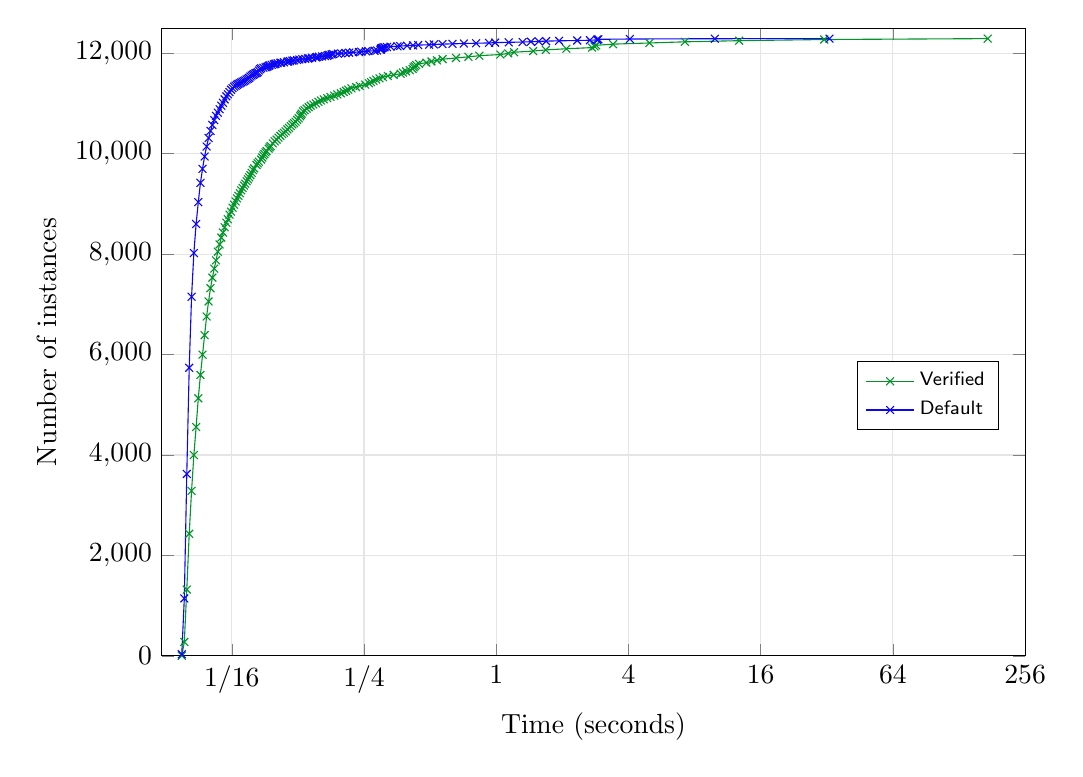
\begin{tikzpicture}[scale = 1.0]
    \begin{axis}
      [
        mark options={scale=1.0},
        grid=both, 
        grid style={black!10}, 
        xmode=log, 
        % ymode=log, 
        legend style={at={(0.97,0.47)}}, 
        legend cell align={left},
        x post scale=1.6, 
        y post scale=1.4, 
        xlabel=Time (seconds), 
        ylabel=Number of instances, 
        xtick={1000/16, 1000/4, 1000, 4000, 16000, 64000, 256000},
        xticklabels={1/16, 1/4, 1, 4, 16, 64, 256},
        xmin=30,
        xmax=256000,
        ymin=0,
        ymax=12500, 
        scaled x ticks=false,
        scaled y ticks=false,
      ]

      \addplot[color=verif, mark=x] coordinates { 
        (37, 3) (38, 277) (39, 1321) (40, 2431) (41, 3286) (42, 3999)
        (43, 4558) (44, 5129) (45, 5595) (46, 5999) (47, 6387) (48, 6759)
        (49, 7059) (50, 7322) (51, 7533) (52, 7712) (53, 7877) (54, 8050)
        (55, 8194) (56, 8331) (57, 8431) (58, 8536) (59, 8626) (60, 8697)
        (61, 8787) (62, 8847) (63, 8926) (64, 8986) (65, 9050) (66, 9110)
        (67, 9161) (68, 9213) (69, 9271) (70, 9319) (71, 9366) (72, 9406)
        (73, 9452) (74, 9490) (75, 9530) (76, 9573) (77, 9621) (78, 9674)
        (79, 9709) (81, 9776) (82, 9810) (83, 9843) (85, 9883) (86, 9926)
        (87, 9966) (88, 9993) (89, 10028) (90, 10054) (92, 10101) (93, 10129)
        (94, 10154) (96, 10206) (98, 10248) (100, 10282) (102, 10321) (104, 10357)
        (106, 10393) (108, 10416) (110, 10446) (112, 10485) (114, 10514) (116, 10550)
        (118, 10584) (120, 10608) (122, 10638) (124, 10674) (126, 10706) (128, 10745)
        (129, 10773) (130, 10800) (132, 10843) (134, 10867) (137, 10898) (140, 10927)
        (143, 10957) (147, 10980) (151, 11005) (155, 11034) (159, 11060) (164, 11083)
        (170, 11108) (176, 11133) (183, 11156) (189, 11181) (196, 11204) (202, 11231)
        (207, 11255) (212, 11278) (219, 11303) (230, 11328) (239, 11351) (253, 11377)
        (263, 11403) (269, 11426) (276, 11452) (284, 11476) (294, 11500) (305, 11525)
        (321, 11548) (341, 11571) (367, 11594) (376, 11617) (389, 11640) (404, 11663)
        (416, 11691) (421, 11721) (426, 11744) (432, 11768) (445, 11791) (481, 11814)
        (507, 11838) (537, 11861) (570, 11884) (656, 11907) (747, 11930) (838, 11953)
        (1044, 11976) (1134, 11999) (1205, 12022) (1473, 12045) (1682, 12068) (2086, 12091)
        (2728, 12114) (2801, 12137) (2853, 12160) (3404, 12183) (4984, 12206) (7225, 12229)
        (12769, 12252) (31142, 12275) (172794, 12293)
      };

      \addplot[color=fast, mark=x] coordinates { 
        (37, 32) (38, 1144) (39, 3623) (40, 5737) (41, 7152) (42, 8022)
        (43, 8602) (44, 9037) (45, 9420) (46, 9699) (47, 9946) (48, 10143)
        (49, 10314) (50, 10454) (51, 10574) (52, 10669) (53, 10755) (54, 10819)
        (55, 10886) (56, 10957) (57, 11015) (58, 11082) (59, 11144) (60, 11186)
        (61, 11228) (62, 11274) (63, 11307) (64, 11335) (65, 11356) (66, 11375)
        (67, 11391) (68, 11404) (69, 11420) (70, 11436) (71, 11446) (72, 11460)
        (73, 11481) (74, 11494) (75, 11511) (76, 11538) (77, 11559) (78, 11573)
        (79, 11584) (80, 11599) (81, 11608) (82, 11625) (83, 11657) (84, 11685)
        (85, 11702) (87, 11712) (89, 11721) (90, 11730) (91, 11738) (92, 11752)
        (93, 11763) (95, 11771) (97, 11779) (98, 11787) (99, 11796) (101, 11802)
        (104, 11809) (105, 11816) (108, 11822) (112, 11832) (113, 11838) (115, 11847)
        (118, 11854) (120, 11860) (124, 11868) (127, 11877) (131, 11883) (135, 11890)
        (139, 11897) (141, 11903) (145, 11911) (151, 11918) (153, 11926) (156, 11932)
        (161, 11938) (166, 11945) (170, 11951) (172, 11962) (174, 11971) (178, 11979)
        (181, 11986) (190, 11993) (197, 11999) (206, 12006) (214, 12013) (223, 12020)
        (237, 12026) (243, 12032) (255, 12039) (262, 12045) (279, 12051) (287, 12057)
        (297, 12069) (298, 12076) (299, 12088) (300, 12099) (301, 12108) (305, 12114)
        (310, 12120) (318, 12126) (330, 12133) (355, 12139) (365, 12146) (393, 12152)
        (418, 12158) (441, 12164) (495, 12171) (520, 12177) (569, 12183) (632, 12189)
        (712, 12195) (810, 12201) (927, 12207) (988, 12213) (1140, 12219) (1318, 12225)
        (1439, 12231) (1561, 12237) (1687, 12243) (1932, 12249) (2338, 12255) (2671, 12261)
        (2877, 12267) (2885, 12273) (2918, 12279) (4059, 12285) (9893, 12291) (32910, 12293)
      };
    
      \legend{
        \scriptsize \textsf{Verified}, 
        \scriptsize \textsf{Default}
      }
    
    \end{axis}
  \end{tikzpicture}

  \caption{
    Runtime comparison between verified and default TESC verifiers. The 
    datapoints of `verified' and `default' show the number of TESC proofs 
    that each verifier could check within the given time limit. The 
    datapoints are not exhaustive; only a subset of them are shown for 
    better visibility.
  }
  \label{fig:chart}
\end{figure}

The performance of VTV was compared against the default TESC verifier 
included in T3P  by running them on all elligible TPTP problems and 
measuring their verification times. A TPTP problem is elligible if it 
satisfies all of the following:
\begin{itemize}
  \item It is in the CNF or FOF language. 
  \item Its status is `theorem' or `unsatisfiable'.
  \item It can be solved by either Vampire or E in one minute using default settings.
  \item The TSTP solution produced by Vampire or E can be compiled to a TESC proof by T3P.
\end{itemize}
If a problem was solved by both Vampire and E and successfully compiled 
by T3P, both of the resulting TESC proof files were used for the test.
There were a total of 12296 elligible problems. Finally, there were 3 
problems that were excluded due to memory constraints, which we will
discuss shortly. The remaining 12293 problems were used for the test.

All tests were performed on Amazon EC2 \texttt{r5a.xlarge} instances, running Ubuntu Server 20.04 LTS on 2.5 GHz AMD EPYC 7000 processors with 32 GB RAM and 512 GB SSD.

The test results are shown in Fig. \ref{fig:chart}. Verification by VTV is
slower than the default verifier, which is expected as the latter is implemented 
with no regard to verification and optimized solely for performance.
In relative terms, the median and mean verification times for VTV were 
1.146 and 3.537 times longer than that of the default verifier, respectively. 
However, the difference in \textit{absolute} terms is small enough that it is 
probably insignificant for most cases: the difference in median times is a
mere 6 milliseconds, and VTV can verify 99.3\% of all proofs under 5 seconds.
So the performance difference should not be an impediment as long as users 
aren't verifying a large batch of proofs or one of the few, hard outliers.

The main downside of VTV is its high memory consumption; VTV failed to check
the aforementioned 5 proofs due to exhausting the 16 GB available RAM.




\section{Conclusion}  \label{sec:conclusion}

what is not verified (parser \& code generation)


\bibliographystyle{plain}

\bibliography{references}

\end{document}

















